\documentclass[hyperref={colorlinks=false},compress,handout,10pt]{beamer}


\newlength{\wideitemsep}
\setlength{\wideitemsep}{\itemsep}
\addtolength{\wideitemsep}{100pt}
\let\olditem\item
\renewcommand{\item}{\setlength{\itemsep}{0.5\baselineskip}\olditem}


\def\LaTeXs{\LaTeX\ }

%\usepackage{tikz}
%\usepackage{pgfplots}

%\usetikzlibrary{arrows,calc}
%%%<
%\usepackage{verbatim}

%\usetikzlibrary{calc,fadings,decorations.pathreplacing,backgrounds}
%% helper macros

%\tikzset{variable/.default=}  

%\tikzset{%
%    add/.style args={#1 and #2}{ to path={%
%    ($(\tikztostart)!-#1!(\tikztotarget)$)--($(\tikztotarget)!-#2!(\tikztostart)$)%
%\tikztonodes},add/.default={.2 and .2}}
%}  


%\tikzset{%
%    >=latex,
%    inner sep=0pt,
%    outer sep=2pt,
%    mark coordinate/.style={inner sep=0pt,outer sep=0pt,minimum size=2pt,
%    fill=black,circle}%
%}



\usetheme{Singapore}
\usecolortheme{lily}
%\usecolortheme[rgb={0,0.17,0.45}]{structure} 
%\usecolortheme[rgb={.855,.647,.125}]{structure} 
\usefonttheme[onlymath]{serif}

%\usepackage{beamerarticle}
\usepackage{listings}
\lstset{
basicstyle=\footnotesize\ttfamily,
%numbers=left,
frame=bottomline,
framextopmargin=50pt,
}


\usepackage{amsmath,amsthm,amssymb}



\usepackage{float}
\floatstyle{boxed}
\usepackage{colortbl}
\usepackage{mathpazo}
\usepackage[small]{eulervm}
%\usepackage[tiling]{pst-fill}
\usepackage{graphicx}
\usepackage{movie15}
\usepackage{bm}
\usepackage{verbatim}
\usepackage{comment}
\usepackage{caption}
\usepackage{subcaption}
\captionsetup[subfigure]{labelformat=empty}
\captionsetup[figure]{labelformat=empty}
%\usepackage[hang,nooneline]{subfigure}
%\usepackage[nooneline]{subfigure}
%\usepackage[OT2,T1]{fontenc}
%\usepackage{pgf,pgfarrows,pgfautomata,pgfheaps,pgfnodes,pgfshade}
%\usepackage{animate}
%\DeclareGraphicsRule{.tif}{png}{.png}{`convert #1 `dirname #1`/`basename #1 .tif`.png}
\graphicspath{{./images/}}
%\renewcommand{\thesubfigure}{}

\newcommand{\mygreen}{\color{green!50!black}}
\newcommand{\myblue}{\color{blue}}
\newcommand{\myred}{\color{red}}
\newcommand{\mycolor}{\color{red}{c}\color{blue}{o}\color{green}{l}\color{orange}{o}\color{cyan}{r}}
\newcommand{\mysize}{\scriptsize{s}\small{i}\normalsize{z}\Large{e}}
\newcommand{\myshape}{\textcircled{s}\textit{h}\texttt{a}\textsf{p}\textsc{e}}

\newcommand{\E}{\mathcal{E}}
\newcommand{\A}{\mathcal{A}}
\newcommand{\mb}{\mathbf}

\newcounter{cnt}
\setcounter{cnt}{0}


%\setbeamercolor*{titlelike}{parent=palette tertiary} 
\xdefinecolor{titlecolor}{rgb}{.855,.647,.125}
%\setbeamercolor{titlelike}{parent=titlecolor}
\setbeamercolor{frametitle}{fg=titlecolor}
\setbeamerfont{frametitle}{series=\bfseries}
%\setbeamercolor{frame title alerted}{use=alerted text,fg=titlecolor,bg=alerted text.fg!75!bg}
%\setbeamercolor{frame title example}{use=example text,fg=titlecolor,bg=example text.fg!75!bg}
%\setbeamercolor{math text}{fg=green!50!black}
\setbeamercolor{normal text in math text}{parent=math text}

\setbeamertemplate{navigation symbols}{} %gets rid of navigation symbols
\setbeamertemplate{footline}[frame number]
\beamertemplateshadingbackground{blue!5}{yellow!10}

\title{{\color{blue} \LARGE 550.400: Mathematical Modeling and Consulting\newline} }

\subtitle{{\color{red} \large Lecture Notes} }

\author{ 
    {\bf{Instructor:}} \\ 
Dr.~N.~H.~Lee \\ 
    \vspace{5pt}
} 
\institute{JHU AMS 2012 FALL}


%\date{\mygreen \today} % \\ Sparks, Nevada}

\date{\mygreen Last Complied on \today} 

\begin{document}

\begin{frame}[plain]
  \titlepage
\end{frame}

\begin{frame}
  \frametitle{Outline}
  \tableofcontents
\end{frame}

\section{Preliminaries}

\begin{frame}
    \frametitle{Syllabus}
    \begin{itemize}
        \item Grade Policy
        \item Attendance
        \item \emph{Tentative} Schedule
        \item Blackboard
        \item Misc.
    \end{itemize}
\end{frame}


\begin{frame}
    \frametitle{What is Mathematical Modeling?}
    \begin{figure}
            \centering
            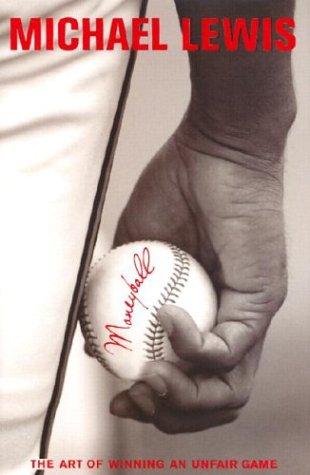
\includegraphics[width=0.4\textwidth]{Moneyballs.jpg}
            \caption{Money Ball}
            \label{fig:MondayBall}
    \end{figure}
\end{frame}

\begin{frame}
    \frametitle{What is Mathematical Modeling?}
    \begin{figure}
        \centering
        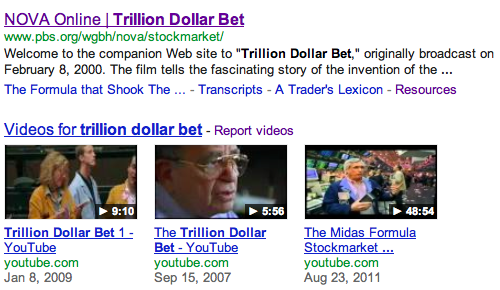
\includegraphics[width=\textwidth]{TrillionDollarBet.png}
        \caption{Trillion Dollar Bet}
                \label{fig:LTCM}
    \end{figure}
\end{frame}

\begin{frame}
    \frametitle{What is Mathematical Modeling?}
    \begin{figure}
        \centering
        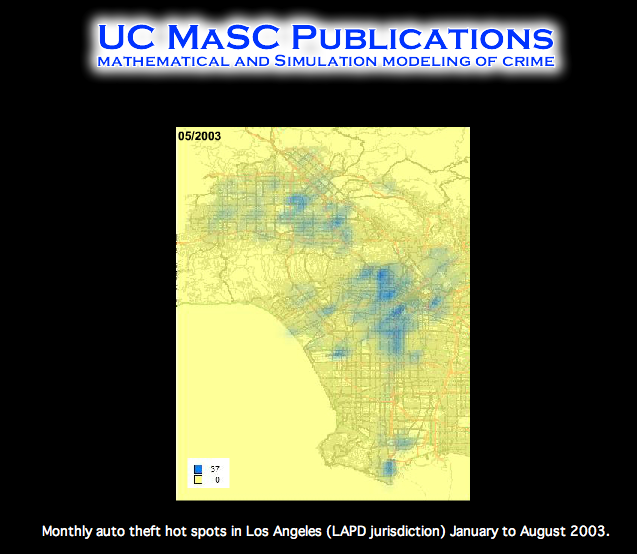
\includegraphics[width=0.6\textwidth]{LAPDUCLA.png}
        \caption{
        \href{http://losangeles.cbslocal.com/video?autoStart=true&topVideoCatNo=default&clipId=6724212}{LAPD Fighting Crime with Math}}
                \label{fig:LAPDUCLA}
    \end{figure}
\end{frame}

\begin{frame}
    \frametitle{What is Mathematical Modeling?}
    \begin{figure}
        \centering
        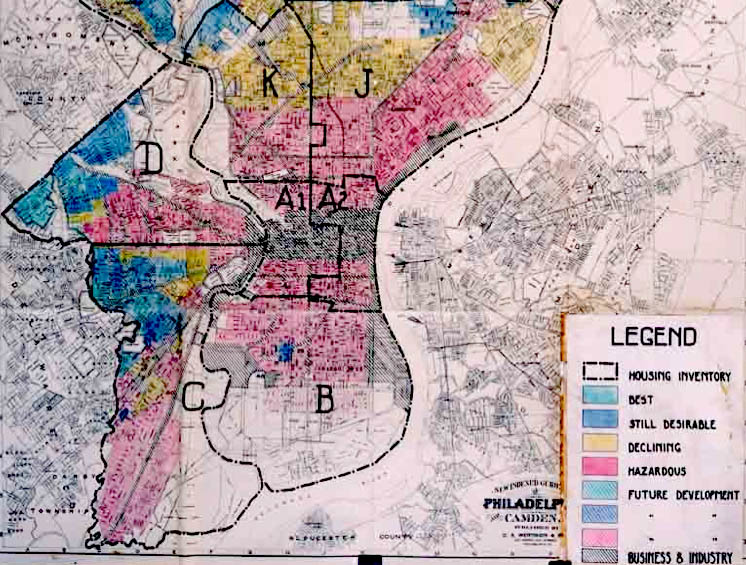
\includegraphics[width=0.8\textwidth]{redliningPhilly.jpg}
        \caption{Insurance Redlining}
                \label{fig:redlining}
    \end{figure}
\end{frame}

\newtheorem{DEFinsredlining}{Insurance Redlining}
\newtheorem{DEFfairplan}{FAIR}
\begin{frame}
    \frametitle{Example: Insurance Redlining}
    \begin{DEFinsredlining}
        \textcolor{red}{Insurance redlining} refers to the practice of refusing
        to issue insurance to certain types of people or within some 
        geographic area. 
    \end{DEFinsredlining}
\vskip.5in
    \begin{DEFfairplan}
        The \textcolor{red}{FAIR} plan was offered by the city of Chicago as a 
        default policy to homeowner who had been rejected by the voluntary
        market. 
    \end{DEFfairplan}
\end{frame}

\newtheorem{DEFsponsorUSCCR}{Sponsor}
\newtheorem{DEFdataFAIR}{Data}
\begin{frame}
    \frametitle{Example: Insurance Redlining}
    \begin{DEFsponsorUSCCR} 
        The \textcolor{red}{U.S.~Commission on Civil Rights} examined 
        charges by several Chicago community organizations that insurance 
        companies were redlining their neighborhoods. 
    \end{DEFsponsorUSCCR}
    \vskip.5in
    \begin{DEFdataFAIR}
        The \textcolor{red}{number of FAIR plan policies} written and renewed in Chicago
        by zip code for the number of months of December 1977 through May
        1978.
    \end{DEFdataFAIR}
\end{frame}

\begin{frame}
    \frametitle{Example: Insurance Redlining}
    Variables to consider:
    \begin{description}
        \item[\texttt{race}] Racial composition in percentage of minority,
        \item[\texttt{fire}] Fire per 100 housing units,
        \item[\texttt{theft}] Theft per 100 housing units,
        \item[\texttt{age}] Theft per 1000 population,
        \item[\texttt{involact}] New FAIR plan policies and renewal per 100 housing units,
        \item[\texttt{income}] Median family income in thousands of dollars,
        \item[\texttt{side}] North or South side of Chicago.
    \end{description}
\end{frame}

\begin{frame}
    \frametitle{Example: Insurance Redlining}
    Frequently Recurring Elements of doing a Project in Industry:
    \vspace{7pt}
             \begin{enumerate}
                 \item Work Statement,
                 \item Midterm Presentation,
                 \item Progress Report,
                 \item Final Presentation,
                 \item Final Report.
             \end{enumerate}
\end{frame}

\begin{frame}
    \frametitle{What is Work Statement?}
    \begin{itemize}
        \item The written proposal and definition of the project
            \vspace{1cm}
        \item Your consulting team's ``contract'' with the sponsor
            \vspace{1cm}
        \item It is ultimately given to the sponsor for review and signature
    \end{itemize}
\end{frame}

\begin{frame}
    \frametitle{What is Work Statement?}
It sets forth: 
    \begin{itemize}
        \item the nature of the project,
        \item the specific objectives of the project, 
        \item the result expected, 
        \item the ``deliverable'' for the project.
    \end{itemize}
\end{frame}

\begin{frame}
    \frametitle{What is Work Statement?}
    \begin{itemize}
        \item The scope of the project must be within the time table for the
            course
            \vspace{1cm}
        \item The deliverables are reasonable and appropriate
    \end{itemize}
\end{frame}
\begin{frame}
    \frametitle{What is Work Statement?}
    \begin{itemize}
        \item Given the nature of research, it should not include promises
            that your consulting team cannot be certain to achieve
        \item It may be necessary after discussion and agreements among
            various parties to modify and renegotiate the work statement as 
            the project progresses
    \end{itemize}
\end{frame}

            
\begin{frame}
    \frametitle{Programmings in this class}
    \begin{itemize}
        \item R:
            \begin{itemize}
                \item \texttt{tikzDevice}
                \item \texttt{lm}
            \end{itemize}
        \item \LaTeXs: 
            \begin{itemize}
                \item \texttt{moderncv}
                \item \texttt{beamer}
                \item \texttt{report}
                \item \texttt{tikz}
            \end{itemize}
        \item Git
            \begin{itemize}
                \item \texttt{git gui}
            \end{itemize}
    \end{itemize}
\end{frame}

\begin{frame}[fragile]
    \frametitle{Demo: R}
    \begin{columns}
        \begin{column}{0.5\textwidth}
    \begin{lstlisting}
install.packages(faraway)
require(farway)
data(eco)
plot(income ~ usborn, 
    data=eco,
    xlab='Proportion US born'
    ylab='Mean Annual Income'
    )
    \end{lstlisting}
        \end{column}
        \begin{column}{0.5\textwidth}
            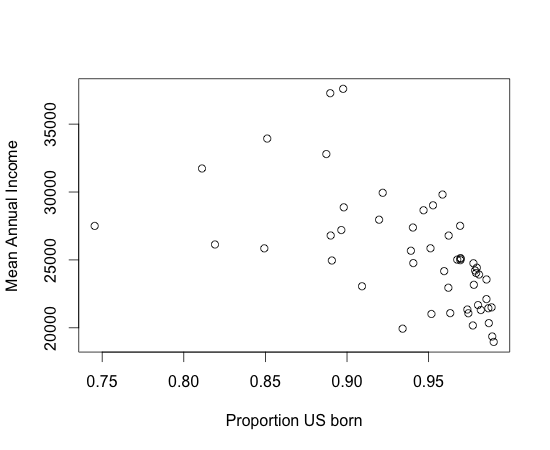
\includegraphics[width=\textwidth]{FigureFarawayFigure11dot1.png}
        \end{column}
    \end{columns} 
\end{frame}

\begin{frame}[fragile]
    \frametitle{Demo: R}
    \begin{columns}
        \begin{column}{0.5\textwidth}
            \begin{lstlisting}
g <- lm(income ~ usborn, eco) 
summary(g)
plot(income ~ usborn, 
    data = eco,
    xlab='Proportion US born',
    ylab='Mean Annual Income',
    xlim=c(0,1),
    ylim=c(15000,70000),
    xaxs='i')
abline(coef(g))
            \end{lstlisting}
        \end{column}
        \begin{column}{0.5\textwidth}
            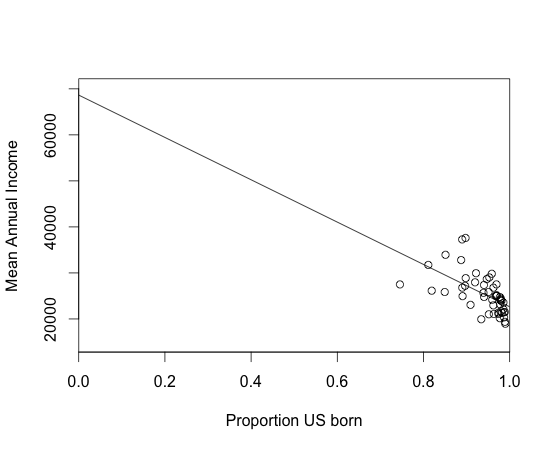
\includegraphics[width=\textwidth]{FigureFarawayFigure11dot1b.png} 
        \end{column}
    \end{columns} 
\end{frame}

\begin{frame}[fragile]
    \frametitle{Tutorial: \LaTeXs}
    \LaTeXs is a computer language for writing a scholarly paper:
    \begin{table}
        \centering
        \begin{tabular}{c|p{3cm}|p{3cm}}
            \quad   &   HTML    & \LaTeXs \\ 
            \hline
            Code    & 
            \begin{lstlisting}
<html> 
 . . .
</html>
            \end{lstlisting} &  
            \begin{lstlisting}
\begin{document}
 . . .
\end{document}
            \end{lstlisting}\\
            \hline
            Complier & Firefox and etc. & pdflatex and etc. \\
            \hline
            Output  & Webpage & PDF file
        \end{tabular}
        \caption{HTML vs \LaTeXs}
        \label{tab:htmlvslatex}
    \end{table}
\end{frame}

\begin{frame}[fragile]
    \frametitle{Tutorial: \LaTeXs}
    \begin{itemize}
        \item Demo on preparing a resume using \LaTeXs \texttt{moderncv} package:
            \begin{itemize}
                \item Install \LaTeXs (MikTex in Windows and MacTex in OSX),
                \item Download \texttt{moderncv} package files from the course folder,
                \item Change file names to reflect you,
                \item Edit the tex file,
                \item Compile using your favorite \LaTeXs editor,
                \item Look at the resulting PDF file.
            \end{itemize}
    \end{itemize}
\end{frame}

\begin{frame}[fragile]
    \frametitle{Tutorial: Git}

\begin{lstlisting}
sudo apt-get install git
\end{lstlisting}

\begin{figure}[b]
    \begin{center}
        
\includegraphics[height=0.6\textheight]{gitguiinstall.png}
    \end{center}
    \caption{An alternative: \texttt{git gui}}
    \label{fig:gitgui}
\end{figure}
    
\end{frame}

\begin{frame}[fragile]
    \frametitle{Tutorial: Git}

\vspace{8pt}
\begin{lstlisting}
cd ~/
git clone http://cis.jhu.edu/~nhlee/550400.git
\end{lstlisting}

\begin{figure}[b]
    \begin{center}
        
\includegraphics[height=0.5\textheight]{gitgui.png}
    \end{center}
    \caption{An alternative: \texttt{git gui}}
    \label{fig:gitgui}
\end{figure}
    
\end{frame}

\begin{frame}[fragile]
    \frametitle{Tutorial: Git}

\begin{lstlisting}
cd ~/550400.git
git reset --hard HEAD
git pull origin master
\end{lstlisting}

\begin{figure}[b]
    \begin{center}
        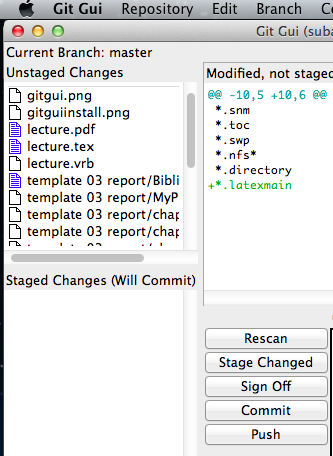
\includegraphics[height=0.65\textheight]{gitguiusing.png}
    \end{center}
    \caption{An alternative: \texttt{git gui}}
    \label{fig:gitgui}
\end{figure}
    
\end{frame}

\begin{frame}
    \frametitle{Tutorial: Git}
    \begin{itemize}
        \item Demo I: build a \emph{personal} Git folder 
            \begin{itemize}
                \item Create some files
                \item Stage the files 
                \item Commit the files
            \end{itemize}
        \item Demo II: build the \emph{course} Git folder
    \end{itemize}
\end{frame}



\section{Principles}
\begin{frame}
    \frametitle{Seven Basic Principles}
     \begin{enumerate}
         \item Set the context 
         \item Choose effective examples and analogies
         \item Choose vocabulary to suit your readers
         \item Decide whether to present \#s in text, tables, or figures
         \item Report and interpret \#s in the text
         \item Specify the direction \emph{and} size of an association between variables
         \item For many \#s, summarize overall pattern 
     \end{enumerate}
\end{frame}


\section{Tools}
\begin{frame}
    \frametitle{Creating Effective Tables}
    
\end{frame}

\section{Arguments from Scale}

\begin{frame}
    \frametitle{Example: Cost of Packaging}
\end{frame}

\section{Graphical Methods}
\begin{frame}
    \frametitle{Example: The Nuclear Mission Arms Race}
    
\end{frame}

\section{Basic Optimization}
\begin{frame}
    \frametitle{Example: Maintaining Inventory}
    
\end{frame}
\end{document}
